%La existencia de la materia oscura es respaldada por muchos fenómenos cosmológicos, de aquí que los investigadores teoricen sobre su composición.

%\subsubsection{Materia oscura bariónica }
En los primeros a\~nos de estudio del problema de la materia oscura en el Universo, se propuso que esta podría ser materia bariónica y otras partículas ligadas a ellos en forma de objetos compactos considerables pero con una emisión electromagnética muy débil. Entre estos candidatos a materia oscura bariónica se encuentran los gases no luminosos, los objetos compactos y masivos de los halos galácticos (MACHOs) y las enanas marrones, sin embargo, múltiples líneas de evidencia contradicen este hecho, ya que contribuyen muy poco a la densidad crítica del Universo.
%La cantidad total de materia oscura bariónica puede ser calculada a partir de la nucleosíntesis del big bang, y las observaciones del fondo de microondas cósmicas. Ambas indican que la cantidad de esta materia es mucho menor que la cantidad total de materia oscura.
%En el caso de la nucleosíntesis, el problema es que una gran cantidad de materia normal significa un universo joven muy denso, es decir, una conversión eficiente de materia a helio-4 y menos deuterio restante. Si asumimos que toda la materia oscura del universo está formada por bariones, entonces hay muchísimo más deuterio en el universo. Esto puede resolverse si hubiera alguna manera de generar deuterio.
%pero se han realizado grandes esfuerzos desde los años 70 con resultado negativo, generalizando la idea de que no puede crearse dicho elemento.

%\subsubsection{Materia oscura no-bariónica} 
Entonces ante la propuesta de que la materia oscura puede estar compuesta por materia no bariónica, esta se puede clasificar en caliente, tibia o fría. Esta clasificación está relacionada con la dispersión de velocidades de la partícula en el momento en que se desacopló del plasma primigenio:
\begin{itemize_f}
\item \textbf{Materia oscura caliente: } aquellas que se mueven \href{https://en.wikipedia.org/wiki/Ultrarelativistic_limit}{ultrarrelativistamente}. Estas hacen referencia a una determinada partícula $\chi$ de masa $m_\chi$ con una velocidad relativista al momento de desacoplarse del plasma primigenio, por lo tanto, su temperatura cumple con la condición $T_\chi \gg m_\chi$. 

\item \textbf{Materia oscura fría :} aquella que no se mueven relativistamente al momento de desacoplarse ($v_\chi \sim 0$), por lo cual $T_\chi \ll m_\chi$. 

\item \textbf{Materia oscura templada o tibia :} aquella que se mueven relativistamente, ella posee características intermedias entre las frías y calientes, o sea, con dispersión de velocidades al momento de desacoplarse mayores a las de la materia oscura fría pero menores a las de la materia oscura caliente.
\end{itemize_f}

Algunos de los candidatos a materia oscura más populares en el área de la física de partículas son: 

\begin{itemize}
\item \textbf{\Axiones}%\footnote{Más información en: \href{https://wikimili.com/en/Axion}{https://wikimili.com/en/Axion}} 
: Esta partícula es el bosón pseudo-Goldstone que resulta del rompimiento espontáneo de la simetría Peccei-Quinn. Esta simetría se postula en 1977 en las extensiones del modelo estándar para resolver el problema de la violación carga-paridad \textbf{CP}\footnote{Se basa en la composición de la simetría \textbf{C} y la simetría \textbf{P}, la primera afirma que las leyes de la Física son invariantes  ante cambios de partículas de carga positiva a negativa y la segunda postula que la invarianza bajo inversiones especulares. } de la interacción fuerte en \QCD. Las observaciones cosmológicas y las mediciones en los aceleradores de partículas acotan la masa del axión a valores de $\lesssim 10^{-2}~\mathbf{eV}$ por lo que cae en la categoría de materia oscura fría. Una de las características de los axiones es que dado que tiene interacciones extremadamente débiles con otras partículas, éstas podrían no estar en equilibrio térmico en el Universo temprano. 

\item  \SUSY (\textbf{SU}per\textbf{SY}mmetry): postula la existencia de una partícula, compañero supersimétrico de las partículas del \ME ~ pero con espín diferente. Esta se presenta como una simetría de tipo espacio-temporal. Una extensión supersimétrica del \ME ~ resuelve los principales problemas de jerarquía dentro de la teoría.

\item \WIMPs ( \textbf{W}eakly \textbf{I}nteracting \textbf{M}assive \textbf{P}articles) %\footnote{Más información en: \href{https://wikimili.com/en/Weakly\_interacting\_massive\_particles}{https://wikimili.com/en/Weakly\_interacting\_massive\_particles}}
: son partículas que se desacoplan siendo no relativistas cuando el Universo tenía una temperatura de $\simeq 1~ GeV$, por lo que caen en la clasificación de materia oscura fría. Las masas
de los \WIMPs ~ abarcan un intervalo de $10 ~ \mathbf{GeV} ~ - ~ 1 ~ \mathbf{TeV}$. Como su nombre lo indica, es un partícula que interactúa débilmente y gravitacionalmente con el resto de las especies del modelo estándar. 



Entre los candidatos se encuentran:
\begin{itemize}
\item 	\LSP (\textbf{L}ightest \textbf{S}upersymmetric \textbf{P}article)%\footnote{Más información en: \href{https://en.wikipedia.org/wiki/Lightest\_supersymmetric\_particle}{https://en.wikipedia.org/wiki/Lightest\_supersymmetric\_particle}}
: es el nombre genérico dado a la más ligera de las partículas hipotéticas adicionales que se encuentran en los modelos supersimétricos. En modelos con conservación de \href{https://es.wikipedia.org/wiki/Paridad\_R}{paridad R}\footnote{{Más información en: \href{https://es.wikipedia.org/wiki/Paridad\_R}{https://es.wikipedia.org/wiki/Paridad\_R}}}, el \LSP ~ es estable; en otras palabras, el \LSP ~ no puede descomponerse en ninguna partícula del \ME~ ya que poseen paridad R opuesta. Algunos ejemplos más conocidos son el sneutrino ligero, el neutralino ligero y el gravitonio.

%Más información en: \href{https://en.wikipedia.org/wiki/Lightest_supersymmetric_particle}{\texttt{https://en.wikipedia.org/wiki/Ligh\-test\_su\-per\-symme\-tric\-\_\-par\-ti\-cle}}.

\item \href{https://en.wikipedia.org/wiki/Kaluza\%E2\%80\%93Klein_theory}{\textbf{LKP} (\textbf{L}ightest {K}aluza-Klein \textbf{P}article) :} son las partículas hipotéticas que cumplen con la teoría de \href{https://en.wikipedia.org/wiki/Kaluza\%E2\%80\%93Klein_theory}{Kaluza-Klein (teoría \textbf{KK})} unificadora de la gravitación y electromagnetismo construida alrededor de la idea de una quinta dimensión más allá de los cuatro habituales del espacio y el tiempo, siendo considerada precursor de la teoría de cuerdas. Algunos de sus candidatos ligeros son el fotón \href{https://en.wikipedia.org/wiki/Kaluza\%E2\%80\%93Klein_theory}{\textbf{KK}} y el neutrino \href{https://en.wikipedia.org/wiki/Kaluza\%E2\%80\%93Klein_theory}{\textbf{KK}}, con masas en la escala $\mathbf{TeV}$ (para mas información, ver referencia \cite{servant_is_2003}).

%\item \textbf{LTP} (\textbf{L}ightest \textbf{T}-odd \textbf{P}article) :

\end{itemize}


\item \href{https://es.scribd.com/document/273103231/Dark-Pion-Particles-May-Explain-Universe-s-Invisible-Matter}{\textbf{SIMPs} (\textbf{S}trongly \textbf{I}nteracting \textbf{M}assive \textbf{P}article\textbf{s}) :} se supone que los piones oscuros interactúan mucho más fuertemente entre sí, se sugiere que en el universo primitivo los piones oscuros habrían chocado entre sí, reduciendo la cantidad de materia oscura, pero a medida que el universo se expande, las partículas colisionarían cada vez con menos frecuencia, hasta ahora, cuando se extienden de manera tan delgada que casi nunca se encuentran. En la nueva hipótesis, los piones de materia oscura están formados por quark de materia oscura que se mantienen unidos por gluones de materia oscura. (Los quarks ordinarios están unidos por gluones normales), en esta propuesta el gluón oscuro tendría masa.
\end{itemize}

En la física de partículas, las partículas supersimetrías son los candidatos más populares para la física de partículas no descubiertas, estás solucionarían de forma elegante muchos problemas actuales en física de partículas de confirmarme ser correcta. Esta simetría hipotética relacionaría las propiedades de los bosones y los fermiones, pero a pesar de todavía estar por ser verificada experimentalmente, es parte fundamental de muchos modelos teóricos, incluyendo la teoría de supercuerdas. 
\begin{figure}[h!]
\centering
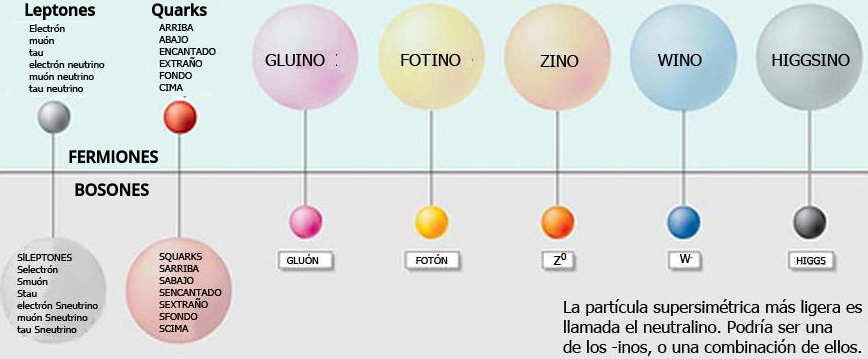
\includegraphics[width=.9\textwidth]{Analisis_y_Resultados/imagenes/supersimetrias.png}
\caption{Extensión del Modelo Estándar bajo la existencia de la supersimetría (\SUSY). %Página de origen : \href{http://www.cienciakanija.com/2009/11/13/confiamos-en-susy-lo-que-realmente-busca-el-lhc/}{\texttt{http://\-www.cienciakanija.com/\-2009/\-11/13/\-con\-fia\-mos-\-en-\-susy-\-lo-\-que-\-real\-men\-te-bus\-ca-el-lhc/}}.
}
\label{susy}
\end{figure}

De forma general el \ME ~se construye a partir de simetrías muy fundamentales que dan lugar a leyes de conservación, en el caso de \SUSY, esta incluye todas las simetrías que ya contiene el \ME~ y añade otra más que involucra al espín. Está teoría postula que a cada partícula del \ME ~le corresponde un compañero supersimétrico que tiene el espín contrario, haciendo que por cada fermión, \SUSY ~añade un bosón y por cada bosón se añade un fermión. Por tanto, el número de partículas predicha es el doble que en el Modelo Estándar, como se visualiza en la Figura~\ref{susy}. Los generadores $\mathbf{Q}$ actúan como:
\begin{equation}
\mathbf{Q}|\mathbf{Fermion}> ~ = ~ |\mathbf{Boson}> ~~~~ \textsf{y} ~~~~ \mathbf{Q}|\mathbf{Boson}> ~ = ~ |\mathbf{Fermion}>
\end{equation}
%Desde su propia definición, este operador tiene dos propiedades de gran alcance:
%\begin{itemize}
%\item Cambia el spin de una partícula y como resultado sus propiedades espacio-temporales. Es por eso que la supersimetría no es una simetría interna sino una simetría de espacio-tiempo.
%\item En una teoría donde se realiza la supersimetría, cada estado de una partícula tiene al menos un supercompañero. Por lo tanto, en un entorno \SUSY, en lugar de estados de partículas individuales, uno tiene que lidiar con (super) múltiplos de estados de partículas.
%\end{itemize}

Se teoriza que \SUSY ~puede dar solución al problema de la materia oscura mediante su teorizada relación con la materia del \ME, en la mayoría de modelos de supersimetría, la partícula supersimétrica más ligera o \LSP ~es necesariamente neutra y estable. %Esto significa que nuestro Universo estaría lleno de estas partículas masivas, neutras y estables, que por tanto serían buenas candidatas a formar la materia oscura.
Sin embargo, debido a que dichas compañeras supersimétricas aún no han podido ser creadas en el laboratorio, sus masas deben ser mucho mayores que las de las partículas originales, implicando que la supersimetría, de ser cierta, está rota por algún mecanismo, la especificación de dicho mecanismo da lugar al Modelo Mínimo Estándar Supersimétrico \MSSM(\textbf{M}inimal \textbf{S}upersymmetric \textbf{S}tandard \textbf{M}odel), que intenta explicar el problema de la materia oscura del universo.





 